\documentclass[a4paper,14pt]{extarticle}

\usepackage[top=1in, bottom=1in, left=1in, right=1in]{geometry}
\usepackage[utf8]{inputenc}
\usepackage[russian]{babel}
\usepackage{graphicx}
\usepackage{caption}
\usepackage{subcaption}
\usepackage{chngcntr}
\usepackage{amsmath}
\usepackage{amsfonts}
\usepackage{pgfplots}
\usepackage{pgfplotstable}
\usepgfplotslibrary{fillbetween}
\usepackage{float}
\usepackage{lipsum}% http://ctan.org/pkg/lipsum
\usepackage{multicol}% http://ctan.org/pkg/multicol
\usepackage{hhline}
\usepackage{tabularx}
\usepackage{tikz,xcolor}
\usepackage{tkz-graph}
\usepackage{float}
\usepackage{mathtools}
\usepackage{todonotes}
\usepackage{listings}
\usepackage[makeroom]{cancel}

\usetikzlibrary{arrows, petri, topaths}

\counterwithin{figure}{section}
\counterwithin{equation}{section}
\counterwithin{table}{section}

\begin{document}
\begin{titlepage}
\centering 
{\bfseries Санкт-Петербургский Политехнический Университет} \\
Институт компьютерных наук и технологий \\
Кафедра компьютерных систем и программных технологий \\
\vspace{5cm}
{\centering \textbf{Отчёт о лабораторной работе 3} \\ 
\vspace{0.2cm}
\textbf{Дисциплина}: Телекоммуникационные технологии \\
\vspace{0.2cm}
\textbf{Тема}: Линейная фильтрация.} \\
\vspace{4cm}
\hfill {\bfseries Работу выполнил:}  \\
\hfill гр. 33501/3 Кнорре А.В. \\
\hfill {\bfseries Преподаватель}  \\
\hfill Богач Н.В.
\vfill
Санкт-Петербург \\
{\large 2018}
\end{titlepage}

\section{Цель работы}
\begin{itemize}
\item Изучить воздействие ФНЧ на тестовый сигнал с шумом. 

\item Сгенерировать гармонический сигнал во временной и частотной областях до и после фильтрации. Сделать выводы о воздействии ФНЧ на спектр сигнала.
\end{itemize}

\section{Ход работы}

\subsection{Преобразование сигналов}

Преобразование непрерывных сигналов в линейных цепях с постоянными параметрами может быть описано с помощью линейных дифференциальных уравнений с постоянными коэффициентами. Результатом интегрирования и дифференцирования гармонической функции некоторой частоты являются также гармонические функции той же частоты. Поэтому при подаче на вход линейной цепи гармонического сигнала, на выходе цепи будет получен гармонический сигнал, отличающийся от входного лишь амплитудой и фазой: 
\begin{equation*}
x(t) = A_x e^{j (2 \pi f t + \varphi x)} ,
\label{f1}
\end{equation*}
\begin{equation*}
y(t) = A_y e^{j (2 \pi f t + \varphi y)} ,
\label{f2}
\end{equation*}

Таким образом частотной характеристикой будет являться отношение выходного сигнала к входному гармоническому сигналу:
\begin{equation*}
G(f) = \frac{y(t)}{x(t)}|_{x(t)}=A_x e^{j(2 \pi f t + \varphi x)} ,
\label{f3}
\end{equation*}
Тогда получаем
\begin{equation*}
G(f) = \frac{A_y}{A_x} e^{j(\varphi_y - \varphi_x)} = |G(f)|e^{j \varphi(f)} ,
\label{f3}
\end{equation*}
где f = y - x. Модуль частотной характеристики G(f) носит название амплитудно-частотной характеристики, а её аргумент f - фазо-частотной характеристики.

\subsection{Фильтры} - это устройства, целенаправленным образом изменяющие спектры сигналов. Фильтрация сигнала, т.е. изменение его спектра, обычно предпринимается с целью увеличить отношение полезного сигнала к шумам и помехам или подчеркнуть (усилить) полезные качества сигнала. Классификация фильтров может быть проведена по различным признакам. 

Признак частотной характеристики делит фильтры на следующие классы:

\begin{itemize}
\item Фильтры нижних частот, подавляющие высокие частоты.
\item Фильтры верхних частот, подавляющие низкие частоты.
\item Фильтры полосно-пропускающие, подавляющие частоты с двух сторон от полосы пропускания
\item Фильтры полосно-заграждающие, подавляющие частоты внутри полосы заграждения
\end{itemize}

\subsection{Simulink}

Сгенерируем синусоидальный сигнал f = 1000 Гц. Наложим на этот сигнал белый шум. 

\begin{figure}[H]
    \centering
    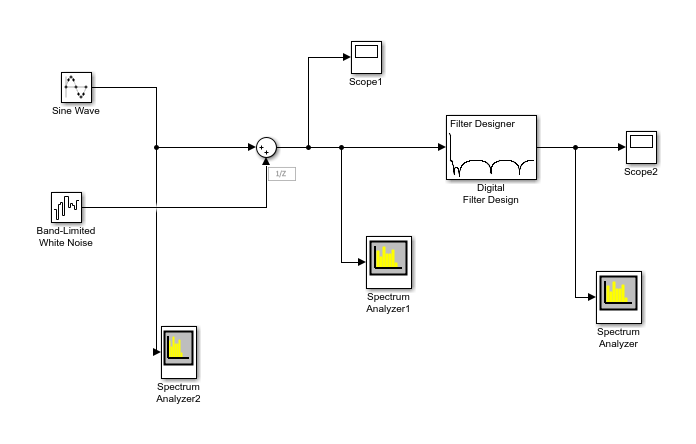
\includegraphics{simulink}
	\captionsetup{justification=centering,margin=1cm}
    \caption{Simulink setup}
    \label{fig:simulink}
\end{figure}

Пронаблюдаем исходный сигнал и его спектр:

\begin{figure}[H]
    \centering
    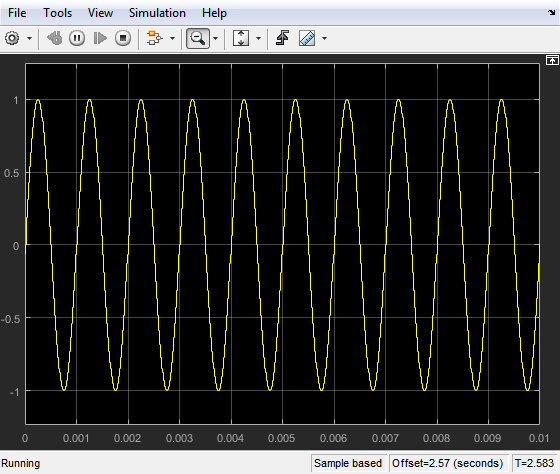
\includegraphics{input}
	\captionsetup{justification=centering,margin=1cm}
    \caption{Input signal}
    \label{fig:input}
\end{figure}

\begin{figure}[H]
    \centering
    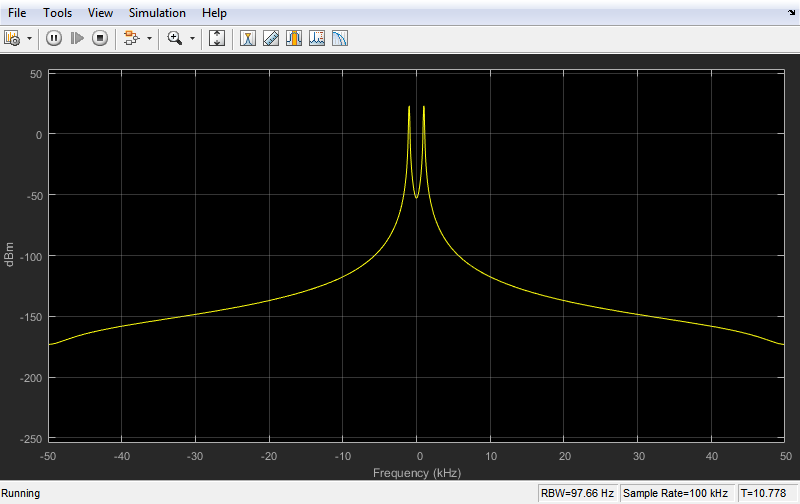
\includegraphics[width=0.95\textwidth]{input_sp}
	\captionsetup{justification=centering,margin=1cm}
    \caption{Input signal' spectre}
    \label{fig:input_sp}
\end{figure}
Посмотрим как изменятся сигнал и спектр после добавления шума:
\begin{figure}[H]
    \centering
    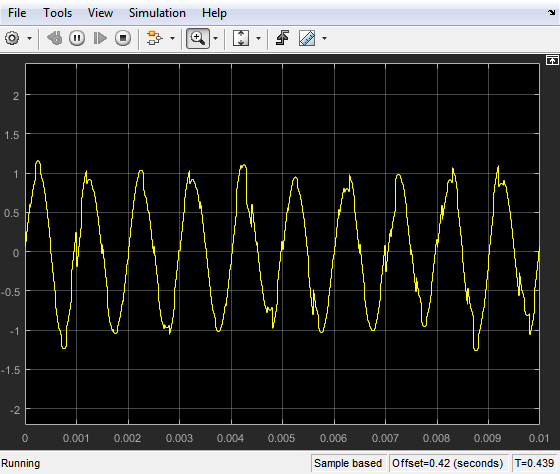
\includegraphics{noise}
	\captionsetup{justification=centering,margin=1cm}
    \caption{Input signal with noise}
    \label{fig:noise}
\end{figure}

\begin{figure}[H]
    \centering
    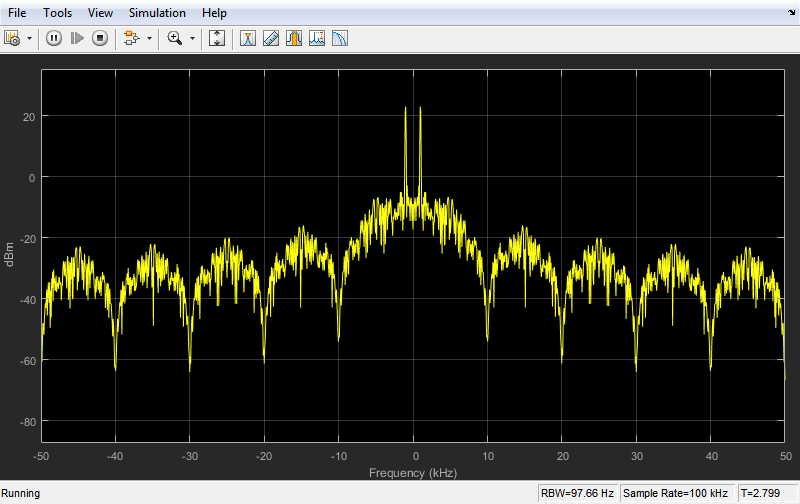
\includegraphics{noise_sp}
	\captionsetup{justification=centering,margin=1cm}
    \caption{Input signal with noise' spectre}
    \label{fig:noise_sp}
\end{figure}
Настроим фильтр таким образом, чтобы пропускать наш исходный сигнал с частотой 1000 Гц и подавлять более высокие частоты белого шума:
\begin{figure}[H]
    \centering
    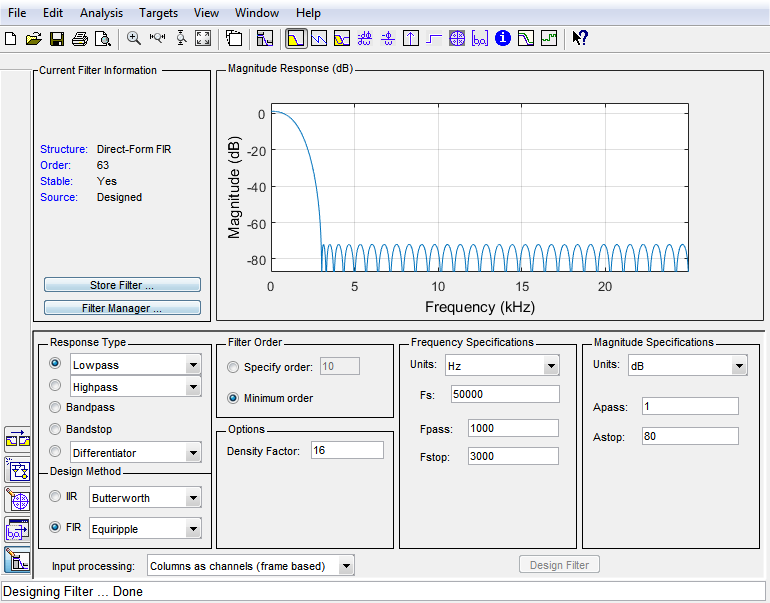
\includegraphics{filter}
	\captionsetup{justification=centering,margin=1cm}
    \caption{Input signal with noise' spectre}
    \label{fig:filter}
\end{figure}

Пропустим зашумленный сигнал через фильтр:
\begin{figure}[H]
    \centering
    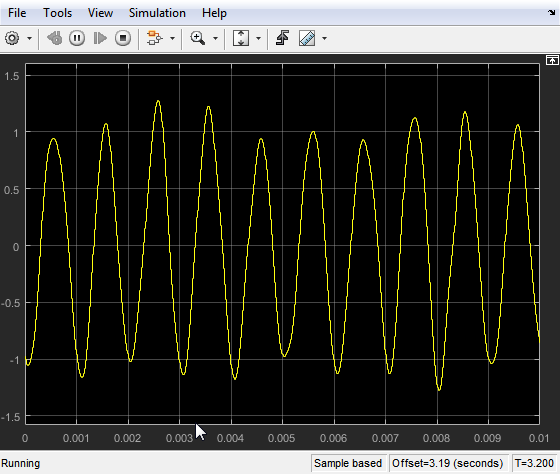
\includegraphics{restored}
	\captionsetup{justification=centering,margin=1cm}
    \caption{Restored signal}
    \label{fig:restored}
\end{figure}

\begin{figure}[H]
    \centering
    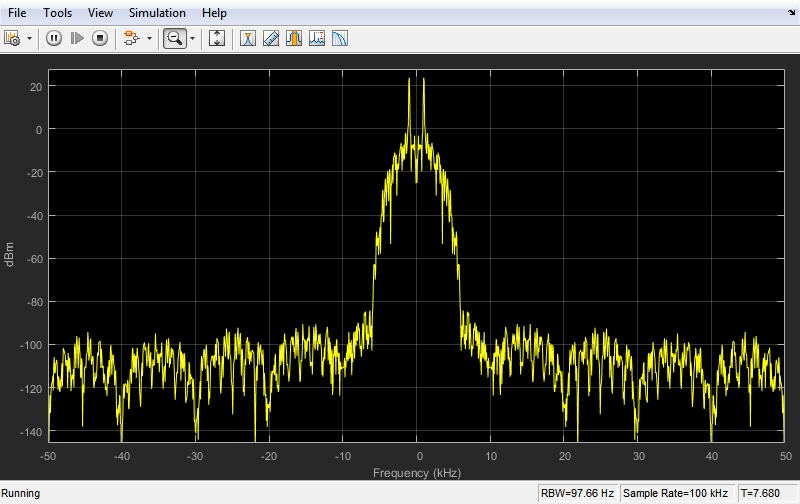
\includegraphics{restored_sp}
	\captionsetup{justification=centering,margin=1cm}
    \caption{Restored signal' spectre}
    \label{fig:restored_sp}
\end{figure}
Видим небольшие искажения, но в целом сигнал восстановлен от помех.

\section{Выводы.}

В данной работе мы воспроизвели синусоидальный сигнал, на который наложили белый шум (помеху). Спектр сигнала также оказался зашумленным. Для восстановления сигнала мы воспользовались фильтром Digital Filter, и подобрав прафильную конфигурацию сумели добиться хороших результатов в восстановлении исходного сигнала после помех (белого шума). Однако высокочастотные помехи по прежнему остаются в востановленном сигнале, что сигнализирует о главной проблеме линейного фильтра.

\end{document}